\documentclass[12pt]{beamer}

\usetheme{metropolis}
\usepackage{appendixnumberbeamer}
\usepackage[utf8]{inputenc}  
\usepackage[brazil]{babel}   

\usepackage{booktabs}
\usepackage[scale=2]{ccicons}

\usepackage{pgfplots}
\usepgfplotslibrary{dateplot}

\usepackage{xspace}
\newcommand{\themename}{\textbf{\textsc{metropolis}}\xspace}

\usepackage{graphicx,url}
\usepackage[table,xcdraw]{xcolor}
\usepackage{pslatex}
\usepackage{scalefnt}
\usepackage[brazil]{babel}   
\usepackage[utf8]{inputenc}  
\usepackage{array}
\usepackage{caption}
\usepackage{subcaption}
\usepackage{float}
\usepackage[defaultmono,scale=.8]{droidmono}



\title{CompactMeter}
\subtitle{Aferição da Compactação do Solo Através de Tecnologias de Sensores e Sistemas Embarcados.}
\date{04 de Julho, 2018}
\author{Guilherme Leonhardt Santa Maria \\ Orientador: Tony Alexander Hild \\ Coorientadores: Mauro Miazaki; Leandro Rampim}
\institute{Universidade Estadual do Centro-Oeste}
\titlegraphic{\hfill\includegraphics[height=1.5cm]{logo.png}}

\begin{document}

\maketitle

\section{Introdução}

\begin{frame}[fragile]{Introdução}

  Evolução tecnológica tem propiciado um grande desenvolvimento na agrícola.
  
  Atualmente a compactação do solo é um dos principais desafios na área.
\end{frame}

\begin{frame}{Introdução}
    Um solo compactado prejudica o desenvolvimento da planta.
    
    Necessário intervenção no local para evitar prejuízos na lavoura.
\end{frame}

\begin{frame}{Introdução}
    Para realizar o calculo da compactação do solo podem ser utilizados diversos métodos.
    
    Um dos métodos é através do índice de patinagem dos rodados do maquinário.
    \begin{itemize}
        \item Cálculo realizado manualmente.
    \end{itemize}
\end{frame}

\begin{frame}{Introdução}
    Sistemas Embarcados tem se beneficiado com o barateamento e a popularização de sensores e plataformas como Arduino e Raspberry Pi.
    
    Otimização do cálculo do índice de patinagem utilizando tecnologias de sistemas embarcados.
\end{frame}

\section{Fundamentação Teórica}
\begin{frame}{Compactação do Solo }
    Um solo compactado tem sua densidade aumentada diminuindo o tamanho e a distribuição dos macroporos \nocite{drescher2011persistencia}.
    \vspace{0.2cm}
    Macroporos são responsáveis pela aeração e drenagem do solo 
    Drescher et al. (2011) \nocite{drescher2011persistencia}.
    \vspace{0.2cm}
    
    Um solo sem compactação possui maior capacidade de absorção de água. Ahmadi e Ghaur (2015). \nocite{ahmadi2015effects}
    
\end{frame}

\begin{frame}{Compactação do Solo}
    Uma das principais causas da compactação é o tráfego intenso de maquinário.
    
    Pode ser intensificada em condições especificas de umidade. 
    
    Nagaoka (2001), Collares et al. (2008), Andrade-Sanchez et al. (2007). \nocite{nagaoka2001desenvolvimento, collares2008compactaccao, andrade2007development}
    
    Veículos leves também podem causas compactação no solo se usados com frequência Ahmadi e Ghaur (2015).
\end{frame}

\begin{frame}{Compactação do Solo}
        A compactação do solo interfere diretamente na eficiência da tração dos eixos mecânicos Gabriel Filho et al. (2010)
        
        Um solo levemente compactado é benéfico para o desenvolvimento de algumas culturas (Nagaoka 2001)
\end{frame}

\begin{frame}{Compactação do Solo}
    Grupos de métodos para avaliar a compactação: (Nagaoka 2001)
    \begin{itemize}
        \item Métodos visuais
        \item Métodos intermediários
        \item Métodos precisos
    \end{itemize}
    
    Métodos de avaliação direta da compactação são custosos Hemmat e Adamchuk (2008). \nocite{hemmat2008sensor}

\end{frame}

\begin{frame}{Sistemas Embarcados}
    Dispositivos com um computador programável projetados visando redução de custos e de produção e de energia.
    
    Dispositivos Móveis facilitam a interação entre sistemas e usuários.
\end{frame}

\begin{frame}{Aplicativos móveis}
    Um aplicativo é composto por diversas \textit{Activity} e \textit{Fragments} Android D. (2018). \nocite{AppActv}
    \begin{itemize}
        \item Em execução.
        \item Completamente sobreposta por outra \textit{Activity}.
        \item Sobreposta por uma \textit{Activity} transparente.
        \item Está pausada ou encerrada
    \end{itemize}
    
\end{frame}

\begin{frame}{Ciclo de Vida}
    \begin{figure}[H]
    \centering
    \includegraphics[scale=.415]{demo/lifecicle.png}
    \caption{Ciclo de vida de uma \textit{Activity}. Android D. (2018)}
    \label{fig:lifecicle}
    \end{figure}
\end{frame}

\begin{frame} {Materiais}
 Software
 \begin{itemize}
     \item Arduino IDE
     \item Microsoft Visual Studio
     \item Xamarin
 \end{itemize}
 Hardware
 \begin{itemize}
     \item Arduino
     \item Giroscópio MPU-605
     \item Módulo Bluetooth HC-05
 \end{itemize}
\end{frame}

\section{Métodos}
\begin{frame}{Métodos}
     Ciclo de desenvolvimento de software Pressman (2016).
     \begin{itemize}
         \item Comunicação
         \item Planejamento
         \item Modelagem
         \item Construção
     \end{itemize}
\end{frame}

\begin{frame}{Métodos}
    Levantamento de materiais necessários e projeto da placa de circuito para ligação entre os componentes.
    
    Soldagem dos componentes em uma placa de prototipagem.
\end{frame}

\begin{frame}{Métodos}
   Teste em um trator para verificar a integridade e resistência do sensor.
    
   Teste simulado para verificar a precisão na leitura do sensor.
   Realizadas 70 rotações em inclinações de $50^{\circ}$, $60^{\circ}$, $75^{\circ}$, $90^{\circ}$, $105^{\circ}$, $120^{\circ}$ e $130^{\circ}$.
\end{frame}

\section{Desenvolvimento}
\begin{frame}{Miniaturização do protótipo}
    Utilizando como base o protótipo desenvolvido durante a programa de Iniciação Científica (PROIC) 2016-2017.
    
    Seleção de componentes e criação de um modelo esquemático utilizado como planta para a criação da Placa de Circuito Impresso (PCB).
\end{frame}

\begin{frame}{Miniaturização do protótipo}
   \begin{figure}[H]
    \centering
    \includegraphics[scale=.6, angle =90]{pcb.png}
    \caption{Design do sensor miniaturizado.}
    \label{fig:pcb}
    \end{figure} 
\end{frame}

\begin{frame}{Modelagem do \textit{case}}
    O primeiro \textit{case} foi desenvolvido de forma que pudesse segurar o sistema e a bateria ao lado
    
    Segundo \textit{case} apresenta pequenas modificações.
    \begin{figure}[H]
    \centering
    \includegraphics[width=\textwidth]{casesAnteriores.png}
    \caption{Designs iniciais de \textit{cases} para o sistema embarcado.}
    \label{fig:caseAnterior}
    \end{figure}
\end{frame}

\begin{frame}{Modelagem do \textit{case}}
    \begin{figure}[H]
    \centering
    \includegraphics[width=\textwidth]{casefinal.png}
    \caption{Design final do \textit{case}.}
    \label{fig:caseAtual}
    \end{figure}
\end{frame}

\begin{frame}{Desenvolvimento do Aplicativo}
    Requisitos:
    \begin{itemize}
    \item Conectar ao sensor via Bluetooth.
    \item Receber e tratar os dados enviados pelo sensor.
    \item Verificar a sua localização atual utilizando dados do GPS.
    \item Calcular a distância percorrida durante uma medição.
    \item Calcular a patinagem do eixo em tempo real.
    \end{itemize}
\end{frame}

\begin{frame}{Desenvolvimento do Aplicativo}
    
\begin{figure}[H]
\centering
\includegraphics[width=\textwidth]{DiagramaClasses.jpg}
\caption{Diagrama de classes do aplicativo.}
\label{fig:classes}
\end{figure}
\end{frame}

\begin{frame}{Desenvolvimento do aplicativo}
    \textit{DeviceListActivity}
        \begin{itemize}
            \item Caixa de diálogo.
            \item Listagem de dispositivos Bluetooth.
            \item Seleção de dispositivo desejado
        \end{itemize}
    \textit{BluetoothServicess}
        \begin{itemize}
            \item Gerencia toda a comunicação com o dispositivo Bluetooth.
            \item \textit{Thread} para receber dados do sensor.
        \end{itemize}
    \textit{DataHandler}
        \begin{itemize}
            \item Recebe o dado lido em forma de vetor de bytes.
            \item Converte para ASCII.
            \item Realiza o tratamento e passa por uma expressão regular para validar.
        \end{itemize}
\end{frame}

\begin{frame}{Desenvolvimento do aplicativo}
    Dados do GPS\begin{itemize}
        \item Plugin GeoLocator
    \end{itemize}
    Cálculo da Distância percorrida:
    \begin{itemize}
        \item Criação de uma \textit{Location} com Latitude e Longitude.
        \item Método \textit{DistanceTo}.
    \end{itemize}
\end{frame}

\begin{frame}{Desenvolvimento do aplicativo}
    \begin{itemize}
        \item \begin{equation}
            perimetro = 2 \times \pi \times r
            \label{eq:perimetro}
            \end{equation}
        \vspace{0.4cm}
        \item \begin{equation}
            patinagem = 100 - \frac{\frac{distancia}{voltas}*100} {perimetro}
            \label{eq:patinagem}
            \end{equation}
    \end{itemize}
\end{frame}

\begin{frame}{Testes}
    \begin{figure}[H]
    \centering
    \includegraphics[scale=.3]{testetrator.png}
    \caption{Sensor acoplado ao eixo do trator}
    \label{fig:testeCampo}
    \end{figure}
\end{frame}

\begin{frame}{Testes}
    \begin{figure}[H]
    \centering
    \includegraphics[scale=.35]{testesimulado.png}
    \caption{Sensor na plataforma de testes simulando a rotação de um eixo}
    \label{fig:testesimulado}
    \end{figure}
\end{frame}

\section{Resultados e Discussões}
\begin{frame}{Miniaturização do protótipo}
    \begin{figure}[H]
    \centering
    \includegraphics[width=\textwidth]{pcbfinal.jpg}
    \caption{Sensor miniaturizado}
    \label{fig:pcbfinal}
    \end{figure}
\end{frame}

\begin{frame}{Modelagem do \textit{case}}
    \begin{figure}[H]
    \centering
    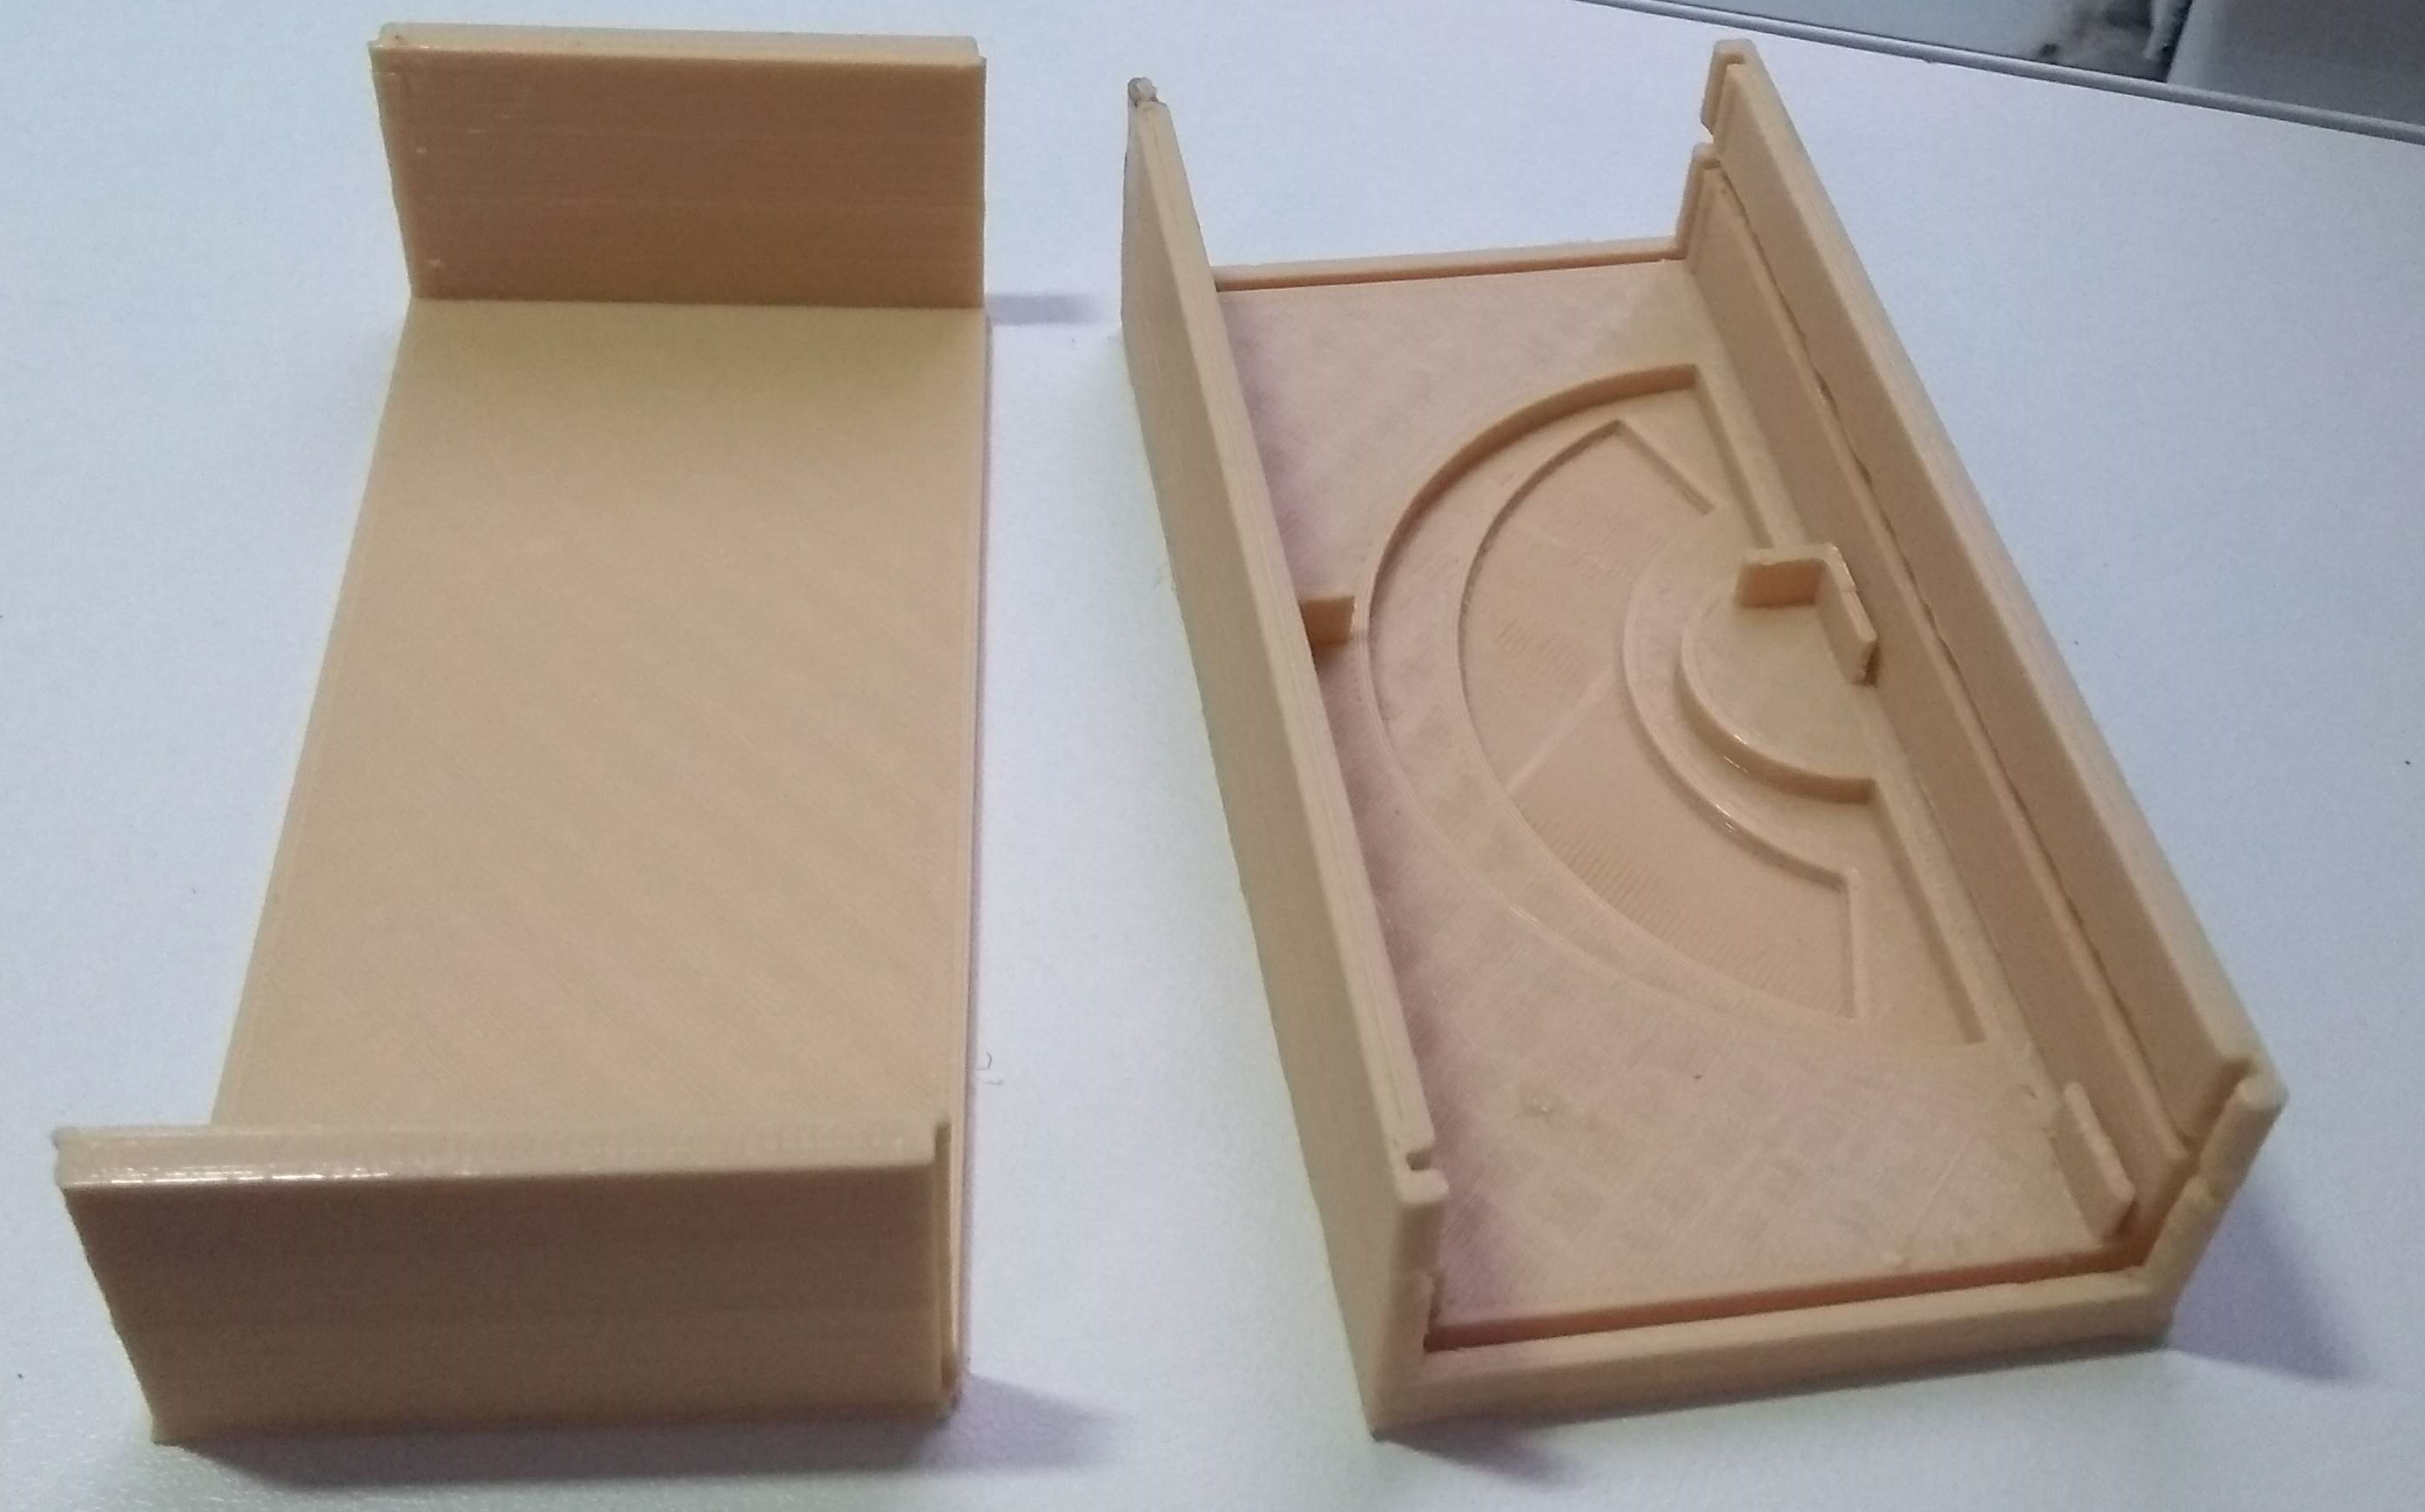
\includegraphics[width=\textwidth]{caseAtual.png}
    \caption{Case para o sistema embarcado impresso em 3D}
    \label{fig:caseImpresso}
    \end{figure}
\end{frame}

\begin{frame}{Desenvolvimento do Aplicativo}
    \begin{figure}
    \centering
        \begin{subfigure}[t]{0.3\textwidth}
        \includegraphics[width=\textwidth]{Main.png}
        \label{fig:RequestEnable}
        \end{subfigure}
        ~
        \begin{subfigure}[t]{0.3\textwidth}
        \includegraphics[width=\textwidth]{DeviceList.png}
        \label{fig:DeviceList}
        \end{subfigure}
        ~
        \begin{subfigure}[t]{0.3\textwidth}
        \includegraphics[width=\textwidth]{medicao.png}
        \label{fig:medicao}
        \end{subfigure}
    \caption{Interfaces do aplicativo CompactMeter}
    \label{fig:interfaces}
    \end{figure}
\end{frame}

\begin{frame}{Testes}
    \begin{itemize}
        \item Conexão estável e resistência.
        \item Necessidade de um case mais resistente.
    \end{itemize}
        \begin{figure}[H]
        \centering
        \includegraphics[scale=.6]{tab.png}
        \caption{Resultado do teste simulado.}
        \label{fig:caseAtual}
    \end{figure}
\end{frame}

\begin{frame}{Considerações Finais}
    Trabalhos futuros:
    \begin{itemize}
        \item Expansão do aplicativo.
        \item Aferição da compactação de um terreno a partir da patinagem.
        \item Criação de formas de visualização gráfica.
    \end{itemize}
\end{frame}

\begin{frame}[standout]
  Obrigado!
\end{frame}

\begin{frame}[allowframebreaks]{References}

  \bibliography{demo}
  \bibliographystyle{abbrv}

\end{frame}

\end{document}
